\section{Zielsetzung}
In diesem Versuch geht es um die Bestimmung der Relaxationszeit $\tau_0$ einer strontiumdotierten Kaliumbromitprobe in Abgängigkeit von der Temperatur. Ebenfalls wird die charakteristische Aktivierungsenergie $W$ für die Diffusion der Leerstellen
untersucht.

\section{Theoretische Grundlagen}

Im Folgenden werden die theoretischen Prinzipien von Polarisationen in Ionenkristallen erläutert und die wichtigen Beziehungen für die Auswertung hergeleitet.

\subsection{Ionenkristalle}
Ionenkristalle beschreiben die periodische Anordnung von verschieden geladenen Atomen (Ionen). Diese sind auf Grund ihrer unterschiedlichen Ladungsvorzeichen vor allem über eine Ionenbindung 
gebunden. Ein idealer Kristall besitzt lokal sowie makroskopisch eine Ladungsneutralität, da die Gesamtbindungsenergie so maximiert wird. In einem reellen Kristall kommt es allerdings in den meisten Fällen auf Grund von 
Unreinheiten durch Wechselwirkung mit der Umgebung,
nur lokal zu Ladungsneutralen Konfigurationen, da die Coulombwechselwirkung vorallem bei kleinen Abständen von Bedeutung ist. Denn es gilt
\begin{equation*}
F_{C} \propto \frac{1}{r^2}.
\end{equation*}
\newline
Nun können ebenfalls weitere Stoffe in den Kristall eingebaut werden. Dieser Prozess wird als Dotierung bezeichnet und ist vor allem dann von Interesse, wenn die Eigenschaften des Kristalls 
beinflusst werden wollen. Die Dotierung von Ionenkristallen mit einem weiteren Ion, welches eine andere Ladung im Vergleich zu den jeweils anderen Basisatomen in dem Kristall hat, sorgt für eine permanente Dipolausbildung.
Ein Beispiel für eine solche Dipolbildung ist anhand einer strontiumdotierten Caesiumiodidkristallstruktur in Abbildung \ref{fig:theo1} angedeutet.
\begin{figure}
    \centering
    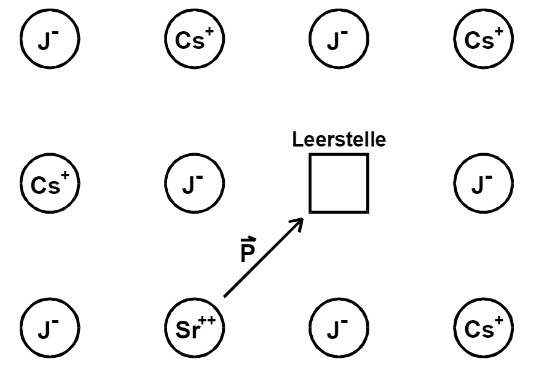
\includegraphics[width=0.6\textwidth]{bilder/theo1.png}
    \caption{Schematische Darstellung einer Caesiumiodidkristallstruktur mit Strontiumdotierung. Zu sehen ist die Dipolbildung $\vec{P}$ zwischen Strontium und Leerstelle. Abbildung nach \cite{altskript}.
            }
    \label{fig:theo1}
\end{figure}
Das Dotierungsmaterial, sowie die Leerstelle, verdrängen hierbei die vorher vorliegenden Gitteratome. Die Einbindung der Leerstellen sorgt für eine lokale Ladungsneutralität. Unterhalb sehr großer Temperaturen sind
sowohl Leerstelle, als auch Strontium, an die diskreten Gitterplätze gebunden. Es liegen somit nur diskrete Dipolmomente $\vec{P}$ vor.
\\
Bei Temperaturen unterhalb $T = \SI{500}{\celsius}$ bewegen sich hauptsächlich die Leerstellen durch den Kristall \cite{altskript}. Somit wird in diesem Versuch nur diese Art von Polarisation berücksichtigt.
Damit es zur Umpolarisation kommt müssen die Leerstellen nun die periodischen Potentialschwellen überwinden können. Die benötigte Energie ist eine charakteristische Größe für die verwendete Probe und 
sie wird Aktivierungsenergie $W$ bezeichnet.

\subsection{Dipolrelaxation und Boltzmann-Statistik}
In einem makroskopischen Kristall der zuvor genannten Art ist die Richtung der vorliegenden Dipole statistisch verteilt, wodurch sich im Mittel ohne äußere Einwirkung ein Gesamtdipolmoment
\begin{equation*}
\sum_{i} \vec{P_{i}} = \vec{0}
\end{equation*}
ergibt. Wird nun als äußere Einwirkung eine Temperatur $T$ der Probe betrachtet, so erhalten die Gitteratome eine thermische Energie die sich aus der Boltzmann-Statistik bestimmen lässt.
Hierbei gilt nun für die Wahrscheinlichtkeit eines Zustandes $n$ nach \cite{Briels2016}
\begin{equation*}
P_n \propto e^{- E_n / k_{B}\text{T}}.
\end{equation*}
Interessant wird es bei Energien $E_n \geq W$, dann haben die Leerstellen genügend Energie um sich im Raum zu bewegen.
\\
Die Relaxationszeit beschreibt nun die Zeit $\tau_0$ zwischen der ersten Umpolarisation des Dipols und der Rückkehr an seine ursprünglichen Stelle.
Somit lässt sich für die Relaxationszeit die folgende Proportionalität erwarten
\begin{equation}
    \label{eqn:lol1}
\tau(\text{T}) \propto  \left( e^{- W / k_{B}\text{T}}\right)^{-1} \quad \to \quad \tau(\text{T}) = \tau_0  e^{ W / k_{B}\text{T}}
\end{equation}
Dabei beschreibt das $\tau_0$ die charakteristische Relaxationszeit.
Die herausgearbeitete Gleichung \eqref{lol1} zeigt dabei schon eine Möglichkeit die Relaxationszeit möglichst groß werden zu lassen. Dies kann in diesem Versuch durch die starke Abkühlung der Probe
erreicht werden, wodurch die Polarisation förmlich \enquote{eingefroren} wird.
\\
Es gibt nun zwei mögliche Herangehensweisen um die Aktivierungsenergie $W$ zu berechnen. Diese sind im Folgenden erläutert.

\subsection{Depolarisationsstrommethode}
\label{sec:strom}
Der Depolarisationsstrom beschreibt den messbaren Strom der bei einer Polarisationsänderung einhergeht. Das E-Feld innerhalb der Probe ändert somit seinen Wert und über einen Kondensator lässt sich der abfließende Strom beobachten.
\\
Wichtig für den Strom stellt der Anteil aller Dipole dar, welche in Richtung des Gesamtdipolmoments zeigen. Werden die Dipole von außen über ein E-Feld in eine bestimmte Richtung ausgerichtet, so entspricht dies genau
dieser. Mathematisch lässt sich dieser Anteil über eine Langevin-Funktion beschreiben. Für sie gilt nach \cite{KROGER201577}
\begin{equation}
L(x) = \text{coth}(x) - \frac{1}{x} \quad \Biggl| \quad x := \frac{|\vec{P}||E|}{k_{B} \text{T}}
\end{equation}
mit der Definition für $x$ aus \cite{altskript}. Für kleine Temperaturen $T$ lässt sich diese Gleichung bis zur zweiten Ordnung Taylorentwickeln.
Es folgt
\begin{equation}
y(\text{T}) = \frac{|\vec{P}||E|}{3k_{B} \text{T}}.
\end{equation}
Nun lässt sich folgende Form einer Stromdichte nach \cite{Fuller} definieren
\begin{multline}
j(\text{T}) \propto \{\text{Anteil der zu Beginn ausgerichteten Dipole} y(\text{T} = \text{T}_P)\} \\ \cdot \{\text{Dipolmoment}\} \cdot \{\text{Relaxationsrate}\}.
\end{multline}
Daraus folgt also
\begin{equation}
j(\text{T}) = y(\text{T}_P) |\vec{P}| \left(\frac{\text{d}N}{\text{d}t}\right).
\end{equation}
Wobei die Rate proportional zur Anzahl der Dipole ist und es gilt
\begin{equation}
    \frac{\text{d}N}{\text{d}t} = - \frac{N}{\tau(\text{T})}.
\end{equation}
Zusammen mit Gleichung \eqref{eqn:lol1} folgt daraus bei einer konstanten Heizrate 
\begin{equation}
b := \frac{\text{dT}}{\text{d}t} = \text{const},
\end{equation}
der folgende Zusammenhang
\begin{equation}
    j \left( \text{T} \right) = \frac{\text{p}^2 \text{E}}{3\text{k}_{\text{b}}\text{T}_{\text{p}}} \frac{\text{N}_{\text{p}}}{\tau_0} \text{exp} \left( -\frac{1}{\text{b}\tau_0} \int^{\text{T}}_{\text{T}_0}  \text{exp} \left( - \frac{\text{W}}{\text{k}_{\text{B}}\text{T'}} \right) \text{dT'} \right) \text{exp} \left(-\frac{\text{W}}{\text{k}_{\text{b}}\text{T}} \right)
    \label{killme}
\end{equation}
Für kleine Temperaturen $\text{T} \approx \text{T}_0$ folgt daraus
\begin{equation}
    \label{eqn:theo5}
    \int^{\text{T}}_{\text{T}_0}  \text{exp} \left( - \frac{\text{W}}{\text{k}_{\text{B}}\text{T'}} \right) \text{dT'} \approx 0 \quad \to \quad j \left( \text{T} \right) \approx \frac{\text{p}^2 \text{E}}{3\text{k}_{\text{b}}\text{T}_{\text{p}}} \frac{\text{N}_{\text{p}}}{\tau_0} \text{exp} \left(-\frac{\text{W}}{\text{k}_{\text{b}}\text{T}} \right)
\end{equation}
Nun kann dieser Ausdruck logarithmiert werden uns es ergibt sich eine lineare Gleichung gegeüber reziproker Temperatur mit Steigung $W$. Es folgt also
\begin{equation}
    \label{eqn:theo6}
\text{ln}(j(\text{T})) = - \frac{W}{k_{B}} \left( \frac{1}{\text{T}}\right) + \underbrace{\text{ln}\left( \frac{|\vec{P}|^2 |E| \text{N}_P}{3 k_B \text{T}_P \tau_0}\right)}_{:= \text{const}}.
\end{equation}

\subsection{Polarisationsmethode}
\label{sec:pola}
Der Unterschied zur vorherigen Methode besteht in der Betrachtung der Gesamtpolarisation $\vec{P}$ des Kristalls. Diese ergibt sich aus dem Gesamtdipolmoment pro Volumeneinheit. Nun wird die Polarisation als 
proportional zur Anzahl der orientierten Dipole angenommen. Hierbei gilt nun wieder
\begin{equation}
    \label{eqn:theo3}
\frac{\text{d}P}{\text{d}t} = - \frac{P(t)}{\tau(\text{T}(t))}.
\end{equation}
Die Änderung der Polarisation führt nun zu einem Strom um den Querschnitt $F$, somit lässt sich schreiben
\begin{equation}
    \label{eqn:theo2}
I(t) = F \frac{\text{d}P}{\text{d}t}.
\end{equation}
Zusammen mit der Randbedingung, dass die Polarisation zum Zeitpunkt $t \to \infty$ wieder auf Null, also einer reinen statistischen Verteilung folgen soll, kann die Gleichung 
\eqref{eqn:theo2} integriert werden und es ergibt sich
\begin{equation}
\int_{t(\text{T})}^{\infty} I(t) \text{d}t = - F P(t).
\end{equation}
Unter Verwendung von Gleichung \eqref{eqn:lol1} und \eqref{eqn:theo3} folgt daraus nun
\begin{equation}
    \label{eqn:idkwhat}
\frac{W}{k_B \text{T}} = \text{ln} \left( \frac{\int_{\text{T}}^{\infty} I(\text{T'}) \text{dT'} }{I(\text{T}) \tau_0 b}\right).
\end{equation}
Das Problem der oberen Integrationsgrenze lässt sich durch die Wahl einer Temperatur $T*$ beheben, diese sollte dabei so groß gewählt werden, dass ab der Temperatur $I(T \geq T*) = 0$ gilt. Unter 
Berücksichtigung von Untergrundraten.

\subsection{Bestimmung der charakteristischen Relaxationszeit}
Für die Bestimmung der charakteristischen Relaxationszeit $\tau_0$ wird Gleichung \eqref{killme} nach $T$ abgeleitet
\begin{equation}
\frac{\partial j}{\partial \text{T}}\biggr|_{\text{T}_{\text{max}}} \stackrel{!}{=} 0.
\end{equation}
Dadurch lässt sich das Maximum $T_{\text{max}}$ bestimmen und in Gleichung \eqref{eqn:lol1} einsetzen und nach $\tau_0$ auflösen. Es folgt
\begin{equation}
\tau_0 = \frac{k_B \text{T}^2_{\text{max}}}{Wb} \cdot \text{exp} \left( - \frac{W}{k_B \text{T}_{\text{max}}}\right).
\end{equation}
% \begin{equation}
% \tau \left( \text{T} \right) = \tau_0  \text{exp} \left(\frac{\text{W}}{\text{k}_{\text{b}}\text{T}}\right) 
% \label{eqn:relaxo}
% \end{equation}

% \begin{equation}
% j \left( \text{T} \right) = \text{y} \left( \text{T}_{\text{p}}\right) \text{p} \frac{\text{dN}}{\text{dt}}
% \label{eqn:dichte}
% \end{equation}

% \begin{equation}
% \text{N}\left( \text{T} \right) = \text{N}_{\text{p}} \text{exp} \left( - \frac{1}{\text{b}} \int^{\text{T}}_{\text{T}_0} \frac{\text{dT'}}{\text{dt}}\right)
% \label{eqn:orientierung}
% \end{equation}



% \begin{equation}
% \end{equation}

% \begin{equation}
% \end{equation}

% \begin{equation}
% \end{equation}